  \documentclass[12pt]{exam}
\usepackage{amsthm} \usepackage{libertine} \usepackage[utf8]{inputenc}
\usepackage[margin=1in]{geometry}
\usepackage{amsmath,amssymb}
\usepackage{multicol}
\usepackage[shortlabels]{enumitem}
\usepackage{siunitx}
\usepackage{float}
\usepackage{steinmetz}
\usepackage{cancel}
\usepackage{graphicx}
\usepackage{pgfplots}
\usepackage{listings}
\usepackage{tikz}
\usepackage{circuitikz}


\pgfplotsset{width=10cm,compat=1.9}
\usepgfplotslibrary{external}
\tikzexternalize

\newcommand{\class}{Electronica para Ciencias} % This is the name of the course 
\newcommand{\examnum}{Tarea 3} % This is the name of the assignment
\newcommand{\examdate}{\today} % This is the due date \newcommand{\timelimit}{}





\begin{document}
\pagestyle{plain}
\thispagestyle{empty}

\noindent
\begin{tabular*}{\textwidth}{l @{\extracolsep{\fill}} r @{\extracolsep{6pt}} l}
	\textbf{\class} & \textbf{Name:} & \textit{Sergio Montoya}\\ %Your name here instead, obviously 
	\textbf{\examnum} &&\\
	\textbf{\examdate} &&
\end{tabular*}\\
\rule[2ex]{\textwidth}{2pt}
% ---

\section*{Primera Pregunta}
En este caso desarrollamos por nodos. Tomando en cuenta que:
\begin{align*}
  I_1 &= \frac{V_A - V_B}{R_S} = \frac{V_S - V_B}{R_S} \\
  I_2 &= \frac{V_B - V_C}{R} = \frac{V_B}{R} \\
  I_3 &= \frac{V_B - V_H}{2R} \\
  I_4 &= \frac{V_C - V_D}{2R}= - \frac{V_D}{2R} \\
  I_5 &= \frac{V_D - V_E}{R} = \frac{V_D}{R} \\
  I_6 &= \frac{V_E - V_F}{2R} = - \frac{V_F}{2R} \\
  I_7 &= \frac{V_F - V_G}{R} = \frac{V_F}{R} \\
  I_8 &= \frac{V_G - V_H}{2R} = - \frac{V_H}{2R} \\
  I_{R_L} &= \frac{0-V_H}{R_L} = - \frac{V_H}{R_L}
.\end{align*}

Por los nodos $C$, $E$ y $G$ sabemos que:
 \begin{align*}
  I_2 &= I_4 \\
  I_5 &= I_6 \\
  I_7 &= I_8
.\end{align*}

Con lo que podemos desarrollar:
\begin{align*}
  I_2 = \frac{V_B}{R} = - \frac{V_D}{2R} = I_4 \to V_D = -2 V_B \\
  I_5 = \frac{V_D}{R} = - \frac{V_F}{2R} = I_6 \to V_D = - \frac{V_F}{2}\\
  I_7 = \frac{V_F}{R} = - \frac{V_H}{2R} = I_8 \to V_F = - \frac{V_H}{2}\\
  V_D = -2 V_B = - \frac{V_F}{2} \to  V_F = 4V_B\\
  V_H = -2 V_F\\
  V_H = -2 \left( 4V_B \right) \\
  V_H = -8 V_B
.\end{align*}

Ahora con el nodo $B$ queda
\begin{align*}
  I_1 = I_2 + I_3\\
  \frac{V_S - V_B}{R_S} = \frac{V_B}{R} + \frac{V_B - V_H}{2R}\\
  V_H = -8 V_B\\
  \frac{V_S - V_B}{R_S} = \frac{V_B}{R} + \frac{9V_B}{2R} = \frac{11V_B}{2R}\\
  \frac{V_S}{R_S} = \frac{11V_B}{2R} + \frac{V_B}{R_S}\\
  V_S = V_B\left( \frac{11R_S}{2R} + 1 \right) \\
  V_B = V_S\left( \frac{2R}{11R_S + 2R} \right) \\
  V_H = - 8 \left( \frac{2R V_S}{11R_S + 2R} \right) \\
  V_{out} = V_H = - \frac{16R V_S}{11R_S + 2R}
.\end{align*}

\section*{Segunda Pregunta}

\begin{enumerate}
  \item En este caso es prudente iniciar definiendo un par de variables que utilizaremos despues:
    \begin{align*}
      \mathbb{Z}_1 = \left( \frac{1}{\mathbb{Z}_{C_1}} + \frac{1}{\mathbb{Z}_{R_1}} \right)^{-1} + \mathbb{Z}_{R_S} \\
      \mathbb{Z}_2 = \left( \frac{1}{\mathbb{Z}_{C_2}} + \frac{1}{\mathbb{Z}_{R_2}} \right)^{-1} = \frac{\mathbb{Z}_{C_2}\mathbb{Z}_{R_2}}{\mathbb{Z}_{C_2} + \mathbb{Z}_{R_2}}
    .\end{align*}

    Ahora bien, por medio de analisis de nodos (que fue realizado en una hoja de papel y que realmente no aporta especialmente mucho el ponerlo en este documento). podemos llegar a:
    \begin{align*}
      V_{out} = - \frac{\mathbb{Z}_2}{\mathbb{Z}_1}V_S\\
      V_{out} = - \frac{\frac{\mathbb{Z}_{C_2}\mathbb{Z}_{R_2}}{\mathbb{Z}_{C_2} + \mathbb{Z}_{R_2}}}{\left( \frac{1}{\mathbb{Z}_{C_1}} + \frac{1}{\mathbb{Z}_{R_1}} \right)^{-1} + \mathbb{Z}_{R_S}}V_S\\
      \mathbb{Z}_2 = \frac{\frac{R_2}{j\omega C_2}}{\frac{1}{j\omega C_2}+ R_2} = \frac{R_2}{\left( 1 + j\omega C_2 R_2 \right) }\\
      \mathbb{Z}_1 = \left( j\omega C_1 + \frac{1}{R_1} \right)^{-1} + R_S = \left( \frac{j\omega C_1 R_1 + 1}{R_1} \right)^{-1} + R_S\\
      = \frac{R_1}{1 + j\omega C_1R_1} + R_S = \frac{R_1 + R_S + j\omega C_1R_1R_S}{1 + j\omega C_1R_1}\\
      V_{out} = - \frac{\frac{R_2}{1 + j\omega C_2R_2}}{\frac{R_1 + R_S + j \omega C_1R_1R_S}{1+j\omega C_1R_1}}\\
    \end{align*}
    \begin{align*}
      V_{out} = - \frac{1 + j \omega C_1R_1}{R_1+R_S - \omega^2 C_1C_2R_1R_2R_S + j\omega C_1R_1R_S + j\omega C_2R_2R_1 + j\omega C_2R_2R_S}\left( V_SR_2 \right) 
    .\end{align*}

    Ahora podemos usar: $V_SR_{2} \implies V_SR_2\phase{0^{\circ}}$

    Con lo que llegamos a:
    \begin{align*}
      \left|V_{out}\left( \omega \right) \right| = - \frac{\sqrt{1^2 + \left( \omega C_1 R_1 \right)^2 } V_SR_2 }{\sqrt{\left( R_1 + R_S - \omega^2C_1C_2R_1R_2R_S \right)^2+\left( \omega C_1R_1R_S + \omega C_2R_2R_1 + \omega C_2R_2R_S \right)^2  } }\\
      P_{V_{out}} = 0 + \arctan\left( \omega C_1 R_1 \right) - \arctan\left( \frac{\omega C_1R_1R_S + \omega C_2R_2 R_1 + \omega C_2R_2R_S}{R_1+R_S-\omega^2C_1C_2R_1R_2R_S} \right) 
    .\end{align*}
    \item

      \begin{figure}[H]
        \centering
        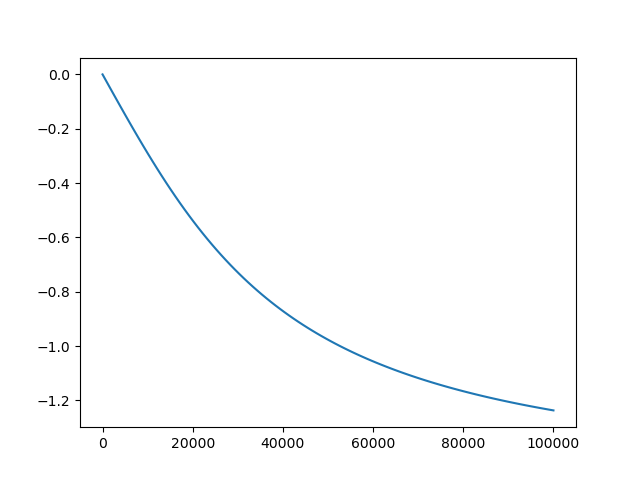
\includegraphics[width=0.8\textwidth]{Graficas/fase.png}
        \caption{Grafica de la fase calculada previamente}
        \label{fig:Graficas-fase-png}
      \end{figure}
    \item 

      \begin{figure}[H]
        \centering
        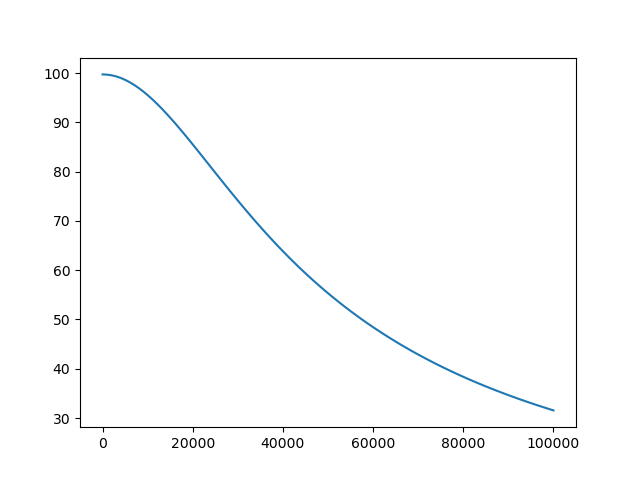
\includegraphics[width=0.8\textwidth]{Graficas/Vout.png}
        \caption{Grafica del voltaje de salida sobre el de la fuente respecto a omega y en valor absoluto.}
        \label{fig:Graficas-Vout-png}
      \end{figure}
\end{enumerate}

\end{document}
